% Start - Hardware/Control Unit/MCU
%write Between the comments

\subsubsection{MCU}
	%Required hardware interfaces
     \textbf{Selecting the \gls{mcu}}
	
	\begin{itemize}
		\item [Step 1:]\emph{ Make a list of required hardware interfaces}\\
		To select a particular \gls{mcu}, the required hardware interfacing is mandatory because hardware interface defines the required peripherals and \gls{gpio}. The list of hardware interface in this project is provided in Table   \ref{tab:mcu_hw_required_interface}(also refer \ref{img:required_hw_interface_mcu}).
		
	\begin{figure}[H]
		\caption{Required Hardware Interface to \gls{mcu}}
		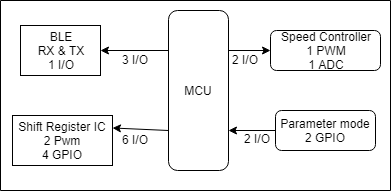
\includegraphics[scale=0.6]{required_hw_interface.png}
		\label{img:required_hw_interface_mcu}
	\end{figure}
	
		\item [Step 2:] \emph{Examine the architecture}\\	
		The project requires fast execution of instruction  and repetitive access to memory due to use of communication protocols and \gls{usart} peripheral. The \textbf{Harvard architecture} suites this application more than the Von-Neuman architecture, since Harvard architecture has dedicated buses for different sections of \gls{mcu} and has pipeline instruction set feature, thus executing  more instructions than Von-Neuman  architecture in a given period of time. 
		The \gls{mcu} should have be either 8 bit or 16 bit, since the application does not require high and complex processing. A 8 bit \gls{mcu} supporting few Mhz of frequency will also suit this application.
		
		\item[Step 3:] \emph{Identify Memory Needs}\\
		This project would require the following minimum memory(as per rough calculations).
			\begin{itemize}
				\item[\acrshort{eeprom} :] 1 \acrshort{kb}
				
				\item[Flash :] 16 \acrshort{kb}
				
				\item[\acrshort{sram} :] 512 Bytes
			\end{itemize}
		
		
		\item[Step 4:] \emph{Searching for \gls{mcu}}\\
		Selecting \gls{mcu} as per above parameters, \gls{avr} series from Atmel crop and MSP40 series of Texas Instruments are good options.considering future enhancement, cost, development kits, support for \gls{mcu} and development platform (like IDE and drivers) the \gls{avr} series ATmega328P is selected. 		 
		 
	\end{itemize}
	
	\textbf{ATmega328P}\\
	 
	   The \gls{mcu} is the central processing unit of the system. For this application/project the ATmega328P, by Atmel Corporation is selcted. Following is the list of features \cite{AtMega328P}.
	 
	 \begin{itemize}
		\item Advanced \gls{risc} architecture
		\item 32K bytes of in-system self-programmable flash program memory.
		\item 1Kbytes \gls{eeprom}.
		\item 2Kbytes \gls{sram}.
		\item Two 8-bit Timer/Counters
		\item One 16-bit Timer/Counter
		\item Six \gls{pwm} channels
		\item 8-channel 10-bit \gls{adc}
		\item \gls{usart}
		\item Master/slave \gls{spi}
		\item \gls{i2c}
		\item watchdog timer
		\item On-chip analog comparator
		\item Six sleep modes 
			
	%	\begin{minipage}{0.3\textwidth}
	%		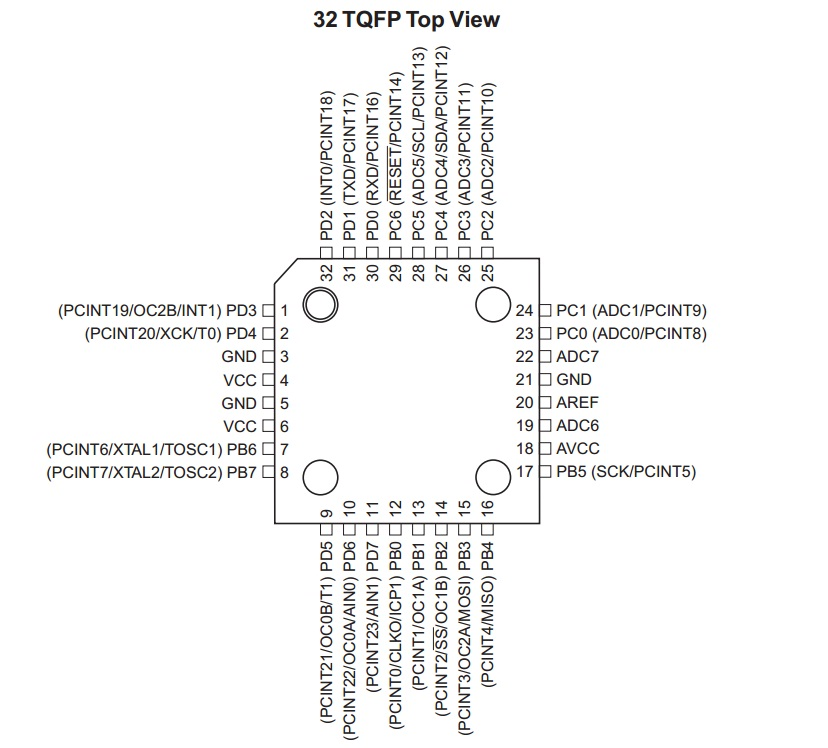
\includegraphics[width=\linewidth]{ATMega328p_TQFP_Pinout.jpg}
			%\caption{Block Diagram V0.21}
		%	\label{fig:image1}
			
		
		%\end{minipage}
		
	\end{itemize}	  
	 
%\begin{multicols}{1}	
	\begin{table*}[t]
		\caption{Required Hardware Interface to \gls{mcu}}	
		\begin{tabular}{l|l|l|l|l|l|l|}
			\hline
			\multicolumn{1}{|l|}{\textbf{Sr. no.}} & \textbf{Interface}        & \textbf{\gls{gpio}} & \textbf{\gls{pwm}} & \textbf{\gls{adc}} & \textbf{\gls{usart}} & \textbf{Remark}                                                             \\ \hline
			\multicolumn{1}{|l|}{\textbf{1}}       & \textbf{\gls{ble}}              & 0             & 0            & 0            & 1              & \acrshort{rx} and \acrshort{tx}                                                                   \\ \hline 
			\multicolumn{1}{|l|}{\textbf{2}}       & \textbf{\gls{ble} \gls{led}}          & 1             & 0            & 0            & 0              & Show \gls{ble} status                                                             \\ \hline
			\multicolumn{1}{|l|}{\textbf{3}}       & \textbf{Speed Control}    & 0             & 1            & 1            & 0              & \begin{tabular}[c]{@{}l@{}}Control scrolling \\ speed\end{tabular}          \\ \hline
			\multicolumn{1}{|l|}{\textbf{4}}       & \textbf{Parameter mode}   & 2             & 0            & 0            & 0              & Edit parameters                                                             \\ \hline 
			\multicolumn{1}{|l|}{\textbf{5}}       & \textbf{Serial Interface} & 0             & 0            & 0            & 1              & \begin{tabular}[c]{@{}l@{}}\acrshort{rx} and \acrshort{tx}\\ Multiplexed with \\ \gls{ble}\end{tabular} \\ \hline
			\multicolumn{1}{|l|}{\textbf{6}}       & \textbf{\acrshort{ic} 74HC595}       & 4             & 2            & 0            & 0              & \begin{tabular}[c]{@{}l@{}}1 Row\\ 2 Col\end{tabular}                       \\ \hline
			                                                               & \textbf{Total}            & \textbf{7}    & \textbf{3}   & \textbf{1}   & \textbf{1}     & \multicolumn{1}{c|}{\textbf{12}}                                            \\ \cline{2-7} 

		\end{tabular}
		\label{tab:mcu_hw_required_interface}
	\end{table*}	 
%\end{multicols}
% End - Hardware/Control Unit/MCU
